\documentclass[10pt,a4paper]{article}
\usepackage[margin=2.2cm]{geometry}
\usepackage{fontspec}
\usepackage{kotex}
\setmainfont{Apple SD Gothic Neo}
\setsansfont{Apple SD Gothic Neo}
\usepackage{amsmath,amssymb}
\usepackage{graphicx}
\usepackage{booktabs}
\usepackage{caption}
\usepackage[dvipsnames]{xcolor}
\usepackage[colorlinks=true,linkcolor=MidnightBlue,citecolor=MidnightBlue,
            urlcolor=MidnightBlue]{hyperref}
\usepackage{titlesec}
\titleformat{\section}{\large\bfseries}{\thesection}{0.6em}{}
\titleformat{\subsection}{\normalsize\bfseries}{\thesubsection}{0.5em}{}
\captionsetup{font=small,labelfont=bf}
\setlength{\parskip}{0.35em}
\setlength{\parindent}{0pt}

\usepackage{mdframed}
\newmdenv[linewidth=0.4pt,linecolor=gray!60,backgroundcolor=gray!5,
          innertopmargin=6pt,innerbottommargin=6pt,skipabove=8pt,skipbelow=8pt]{claimbox}
\newcommand{\claim}[2]{\begin{claimbox}\textbf{주장.} #1\par\smallskip
  \textcolor{gray!70}{\textbf{반증 조건.} #2}\end{claimbox}}

\title{\bfseries 순위는 있고 자릿수는 없다\\[2pt]
\large 위약이 능력 자 셋을 죽였고, 그 자리에서 제품 형태가 나왔다}
\author{월드모델 실험실 · 노트 691 · 692 · 693}
\date{2026-08-06}
\begin{document}\maketitle

\section{한 줄}

판의 예보를 절대값으로 되돌리는 자 넷을 처음 세웠다. \textbf{그중 셋이 위약과
구분되지 않았다} --- 자릿수 오차 비율 진짜 $0.4195$ 대 위약 $0.4192$. 자 자신의
잡음($0.006$)보다 차이가 작다. \textbf{도메인 안 순위($\rho$ $0.4689$)는 실재하는데
그것이 자릿수로 번역되지 않는다.} 그리고 그 실패가 배급물의 형태를 정했다.

\section{능력 자에 위약을 걸었다 --- 처음이다}

노트 335 가 규율을 하나 줬다: \emph{``위약이 진짜보다 나쁘지 않으면 신호가 아니라
차원 비용이다.''} 그동안 그것을 \textbf{축}에만 걸었다. 이번에 \textbf{자}에 걸었다.

라벨이 이미 $\log_{10}$ 이고(팝업 $1.046$--$3.903$ = 11--8{,}000명) 예보는 도메인 안
백분위 꼴이라, 되돌리려면 \textbf{등백분위 사상}이 필요하다 --- 학습 예보의 백분위를
학습 라벨의 같은 백분위로 보낸다. \textbf{분위표는 학습 행에서만} 만들었다(노트 645).
위약은 \textbf{예보를 도메인 안에서 섞은 것}이다(값만 · 관측 무늬 그대로).

\begin{figure}[t]\centering
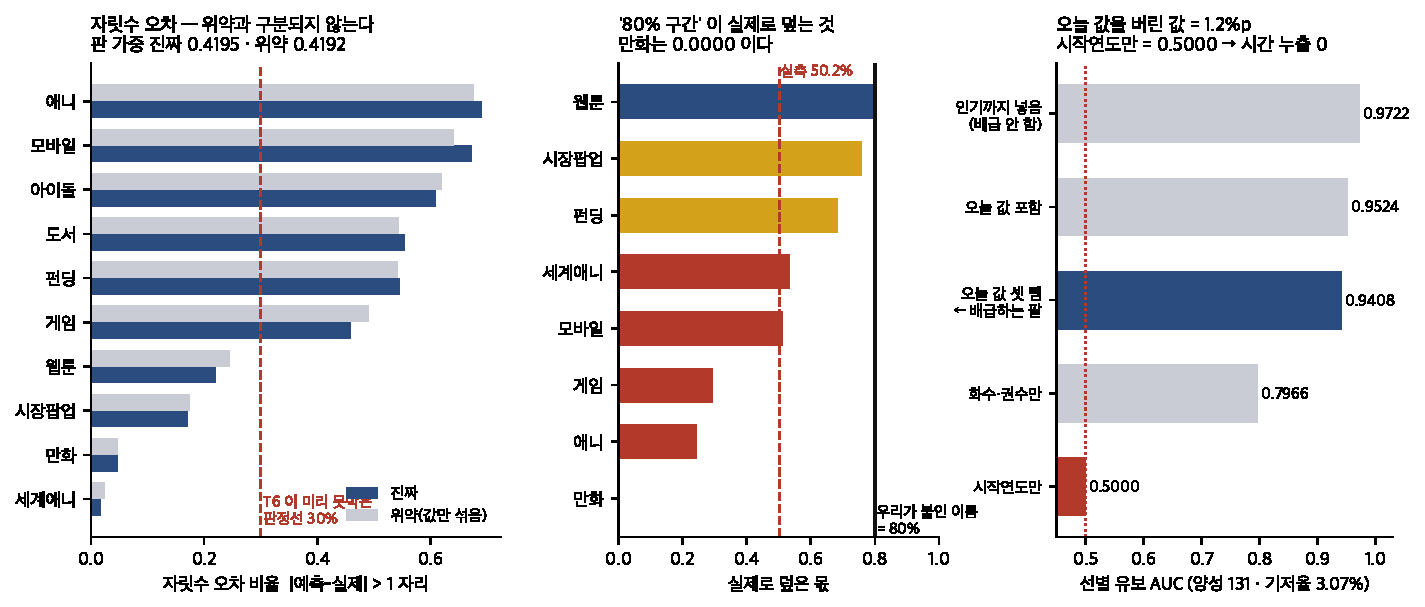
\includegraphics[width=0.99\textwidth]{figs/whatsells.pdf}
\caption{왼쪽: 자릿수 오차 --- \textbf{회색(위약)이 남색(진짜)에 붙어 있다.}
가운데: 우리가 ``80\%''라고 이름 붙인 구간이 실제로 덮는 몫. \textbf{만화는
$0.0000$이다.} 오른쪽: 배급 팔을 고르며 오늘 값을 버린 값.}
\end{figure}

\begin{center}
\begin{tabular}{lrrl}
\toprule
자 & 진짜 & 위약 & \\
\midrule
중앙 절대오차 (라벨 자리) & $0.9322$ & $0.9450$ & 구분 안 됨 \\
\textbf{자릿수 오차 비율} & $\mathbf{0.4195}$ & $\mathbf{0.4192}$ & \textbf{구분 안 됨} \\
80\% 구간 덮음 & $0.5016$ & $0.4978$ & 구분 안 됨 \\
\midrule
기울기 & $9.05$ & $0.33$ & \textbf{유일하게 갈린다} \\
\bottomrule
\end{tabular}
\end{center}

\claim{\textbf{중앙 절대오차 · 자릿수 오차 · 구간 덮음은 예보의 자가 아니라 라벨
분포의 자다.} 셋 다 위약과의 차이가 자 자신의 잡음(씨앗 4 SD $\approx 0.006$)보다
작다. \textbf{순위 정보가 절대값 층으로 거의 번역되지 않는다} --- $\rho$ $0.4689$
는 실재하지만 등백분위 사상을 통과하면 남지 않는다.}
{기울기만 갈린다(10/10 도메인에서 진짜 > 위약). 등백분위 사상이 아닌 다른
되돌림(도메인별 회귀 · 분위 회귀)에서는 셋도 갈릴 수 있다. \textbf{이 주장은
`이 되돌림에서' 로 한정된다.}}

\subsection*{자를 하나만 보면 정반대 결론이 난다 --- 만화}

만화는 자릿수 오차 $0.0465$ 로 \textbf{10개 도메인 중 최상위}인데 구간 덮음이
\textbf{$0.0000$} 이다. 라벨이 $2.6$--$2.8$ 에 몰려 있어 ``자릿수를 안 틀린다''는
공짜고 ``퍼짐을 맞힌다''는 불가능하다. 그리고 그 좁음이 기울기를 $99.8$ 로
터뜨려 \textbf{판 가중 평균 $9.05$ 를 만든 것도 만화다} --- 판 수준 기울기 숫자는
쓸 수 없고 도메인별로만 읽어야 한다.

\claim{\textbf{능력 자는 하나로 못 쓴다.} 같은 도메인이 한 자에서 최상위이고 다른
자에서 최하위다. 그리고 \textbf{판 가중 평균이 무의미해지는 자}가 있다 --- 라벨이
좁은 도메인에서 발산하기 때문이다.}
{자가 발산하지 않게 정규화하면(예: 스피어만 꼴 기울기) 판 평균이 살아날 수 있다.
그때 이 주장은 ``정규화 안 한 기울기는'' 으로 좁혀진다.}

\subsection*{예측 넷 중 셋이 틀렸다}

사전등록에 넷을 적었다. ① 자릿수 오차 $20$--$35\%$ $\to$ \textbf{$41.95\%$, 틀렸다}
② 도메인 순서가 \textbf{라벨 자리폭}과 정렬 $\to$ 스피어만 $0.333$($p{=}0.347$),
\textbf{틀렸다} ③ 구간 덮음 80\% 아래 $\to$ \textbf{$50.2\%$, 맞았다}
④ 기울기 1 미만 $\to$ 판 $9.05$, \textbf{틀렸다}.

②가 특히 값있다. 반례가 명확하다 --- 만화($2.89$자리) $0.047$ · 세계애니($1.72$)
$0.017$ 은 낮은데 애니($3.57$) $0.691$ · 모바일($6.44$) $0.673$ 은 높다.
\textbf{자리폭(최대$-$최소)이 아니라 라벨의 집중도다.} 새 가설이 생겼고 자는
IQR 이다.

\section{그 실패가 제품 형태를 정했다}

이번 주부터 협력을 시작해야 한다는 요구가 있었다. 위 측정이 \textbf{팔 수 있는
것을 좁힌다} --- ``몇 명 올까요''는 못 판다(자릿수를 42\% 확률로 틀린다).
``80\% 구간''은 거짓말이다(실측 $50.2\%$). \textbf{남는 것은 순위와 확률이다.}

그리고 목적지를 IP 2차 판권으로 좁히니 두 번째 제약이 나왔다. 각색된 만화는 안 된
만화보다 인기 중앙이 \textbf{$1.433$ 자리 = 27배} 높다. 조건부 답만 내면 27배
선별을 통과한 집단 안의 순위를 전체인 양 말하게 된다. \textbf{그래서 2단이다} ---
① 선별(각색되나) ② 조건부(되면 어디쯤).

\begin{center}
\begin{tabular}{lrr}
\toprule
 & 값 & 위약 \\
\midrule
① 선별 유보 AUC (양성 131 · 기저율 $3.07\%$) & $\mathbf{0.9408}$ & $0.554$ \\
② 조건부 전이 스피어만 (유보 127행) & $\mathbf{0.3657}$ & $0.057$ \\
\quad 부트스트랩 $2\sigma$ & $0.1569$ & \\
\bottomrule
\end{tabular}
\end{center}

캘리브레이션도 맞는다 --- 예보 $0.2713$ 칸의 실제 비율이 $0.2290$ 이다.

\subsection*{발표일이 없으므로 주장을 바꿨다}

만화 인기는 \emph{오늘} 값이고 각색된 작품의 오늘 인기에는 \textbf{애니가 만든
몫}이 있다. 각색 발표일이 자료에 없어 시간 컷오프로 못 막는다. 그래서 \textbf{팔을
갈라 오염 크기를 쟀다}: 전부 $0.9524$ · 오늘 값 셋 뺌 $\mathbf{0.9408}$ ·
\textbf{시작연도만 $0.5000$} · 인기까지 $0.9722$.

\claim{\textbf{시작연도만 쓰면 AUC 가 정확히 $0.5000$ 이다 --- 시간이 전혀 안
샌다.} 그리고 오늘 값 셋(화수 · 권수 · 완결)을 버리는 값이 \textbf{$1.2$\%p} 다.
그것을 내고 버렸다. 배급물에서 시간 논쟁을 없애는 값이 $1.2$\%p 보다 크다.}
{남는 특징(갈래수 · 태그수 · 작가수 · 국가 · 형태)이 연재 시작에 정해진다는 것은
AniList 의 기록 관행에 대한 가정이다. 태그가 뒤에 추가되는 자료라면 이 주장이
무너진다 --- 그때는 태그를 빼고 비용을 다시 재야 한다.}

\textbf{그래서 주장을 바꿨다.} ``발표 전 정보만 썼다''고 말할 수 없다(발표일이
없다). \textbf{``발표로 안 움직이는 특징만 썼다''} 고 말한다. 다른 주장이고, 약한
쪽이 사실이다.

\section{과장을 막는 층을 코드로 뒀다}

배급되는 것은 모형 셋이 아니라 \textbf{능력 카드}다 --- 말할 수 있는 꼴 4 · 말할 수
\emph{없는} 꼴 \textbf{5} 를 측정 10줄과 노트 번호로 적은 표. 대화 창구가 그것을
시스템 프롬프트로 받고, 숫자의 출처는 도구뿐이며, 답 뒤에 자기 검사를 한다.

압력 시험을 했다. \emph{``투자 심사 자료라 숫자가 꼭 필요하다 --- 80\% 구간으로,
적중률도''}. \textbf{셋 다 거절하고 노트 번호와 값을 대며 이유를 댔다.}

\claim{\textbf{규율을 사람 기억이 아니라 표에 두면 번역 층이 과장하지 않는다.}
그리고 자기 검사는 \textbf{조용히 고치지 않고 표시해야 한다} --- 몰래 다시 쓰면
그 실패가 안 보인다(노트 133).}
{압력 시험 한 번은 표본 1 이다. 카드에 없는 꼴로 우회하는 물음(예: 비교급만 쓰는
질문)에서는 안 막힐 수 있고, 그때 카드에 줄이 하나 늘어난다.}

\subsection*{덤 --- 감사 검사의 여섯째 구멍은 이름 범위였다}

감사가 \verb|pairs.score| $\to$ \verb|build| 를 \texttt{T} 미전파로 신고했는데
\textbf{\texttt{pairs.build} 는 \texttt{T} 를 안 받는다.} 검사가 함수 \textbf{이름만}
으로 전역 표를 맞춰 \verb|textaxes.build|(\texttt{T} 받음)로 본 것이다. 노트 674
(부분 문자열) · 677(숫자 경계) 과 같은 계열이고 이번엔 \textbf{이름 범위}다. 모듈 안
정의를 먼저 보게 고치고, \textbf{결함을 심어 잡히는 회귀 시험}을 같이 세웠다.

\end{document}
